\chapter{Results}
\label{chap:results}

% Talk about the calculations we did: parameters as before described with variable \lambda_{ir}; mean phonons, projections, see appendix A, etc...

\section{Classification of the excitations}
\label{sec:classification}

As previously noted in section \ref{sec:hamiltonian-and-basis}, only for zero electron-lattice couplings the eigenstates of the many-body Hamiltonian (\ref{eq:full-hamiltonian}) can be described as a direct product of purely electronic and phononic states. 
In that scenario each eigenstate has a sharp value for the phonon number operators $b_Rb^\dagger_R$ and $b_{ir}b^\dagger_{ir}$ allowing its identification as a \textit{phononic} state with a given number of phonons (an eigenstate of $H_{ph}$), an \textit{electronic} state (an eigenstate of $H_{el}$) or a product of those two.
However, for electron-lattice couplings larger than zero, the phonon number operator has some dispersion and the eigenstates are no longer purely phononic or electronic in nature.
In figure \ref{fig:electr-proj} we show the first electronic state for different $\lambda_{ir}$ values

%% \begin{figure}[ht!]
%%   \centering
%%   \includegraphics[width=0.5\textwidth]{images/electronic-state-projections.png}
%%   \caption{Electronic state projected...}
%%   \label{fig:electr-proj}
%% \end{figure}


% - Following the eigenvalue, mean ir (Ram) and their dispersions we can track them with increasing coupling (plot?)
% Maybe include the plot projecting the electronic state at \lambda_{ir}>0 with itself at \lambda_{ir}=0


Section about the states with 2 and 3 infrared phonons and their particular behaviour.

\section{Energy renormalization}

At large $\lambda_{ir}$ we recover the harmonic behaviour. This is analog to have a spring with a displaced equilibrium position.

\section{Projection into phonon coordinates}

State with two infrared phonons:

\begin{figure}[ht!]
  \centering
  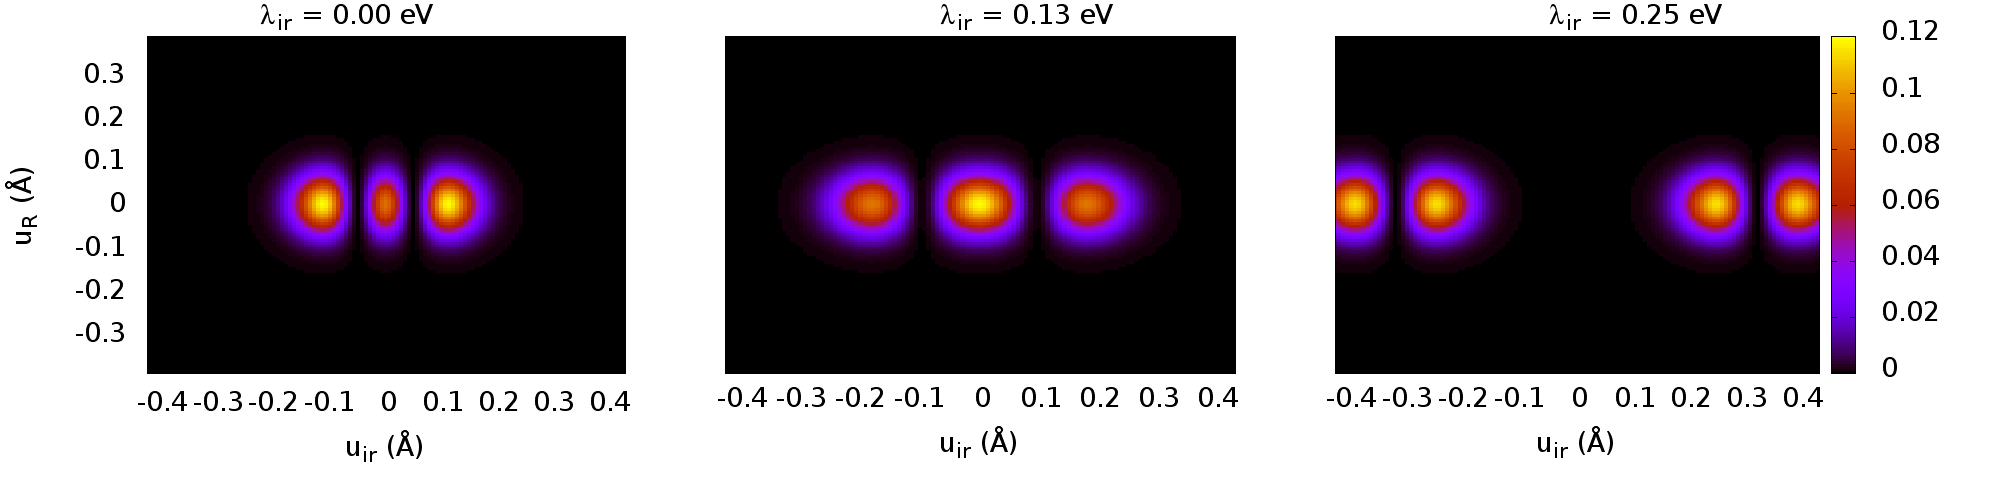
\includegraphics[width=0.8\textwidth]{images/ph-second_infrared.png}
  \caption{Projection into phonon coordinates of the state with 2 infrared phonons.}
  \label{fig:ph-second_infrared}
\end{figure}

State with three infrared phonons:

\begin{figure}[ht!]
  \centering
  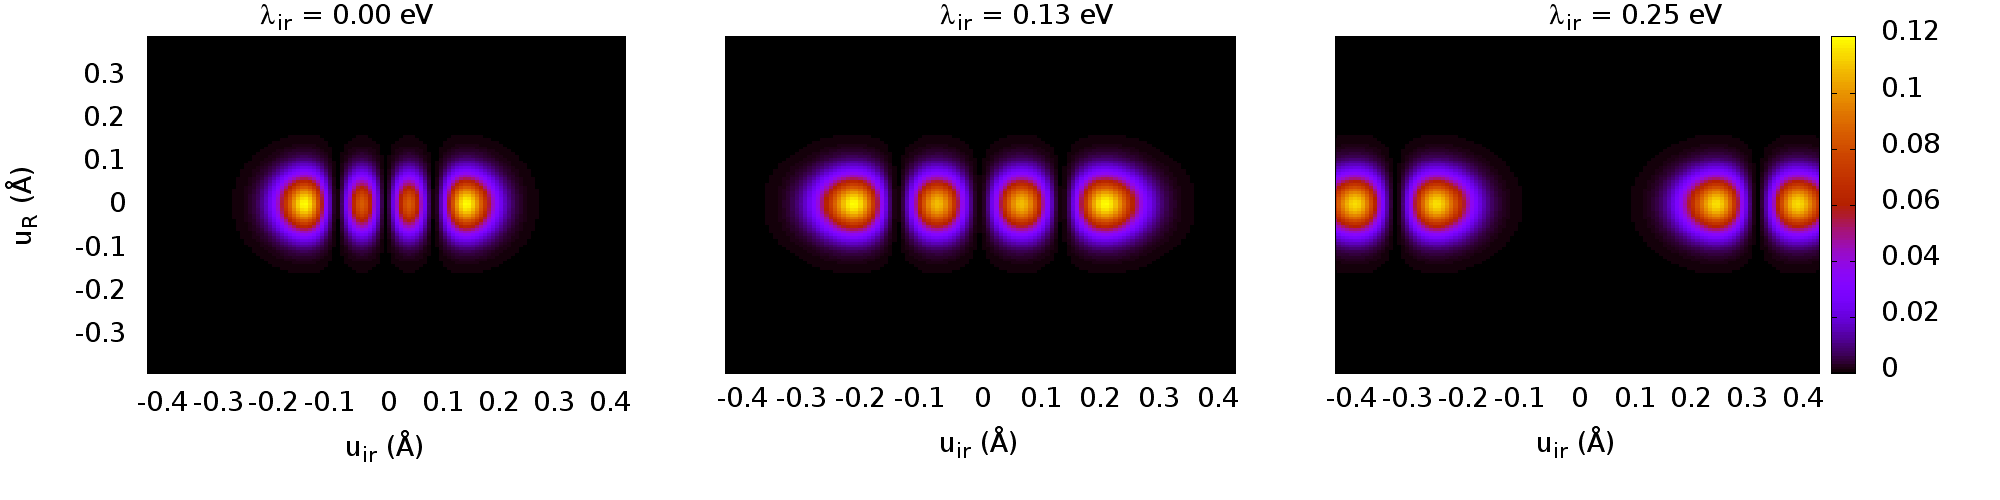
\includegraphics[width=0.8\textwidth]{images/ph-third_infrared.png}
  \caption{Projection into phonon coordinates of the state with 3 infrared phonons.}
  \label{fig:ph-third_infrared}
\end{figure}

\section{Isotopic shifts}

The isotopic shifts are different:

\begin{figure}[ht!]
  \centering
  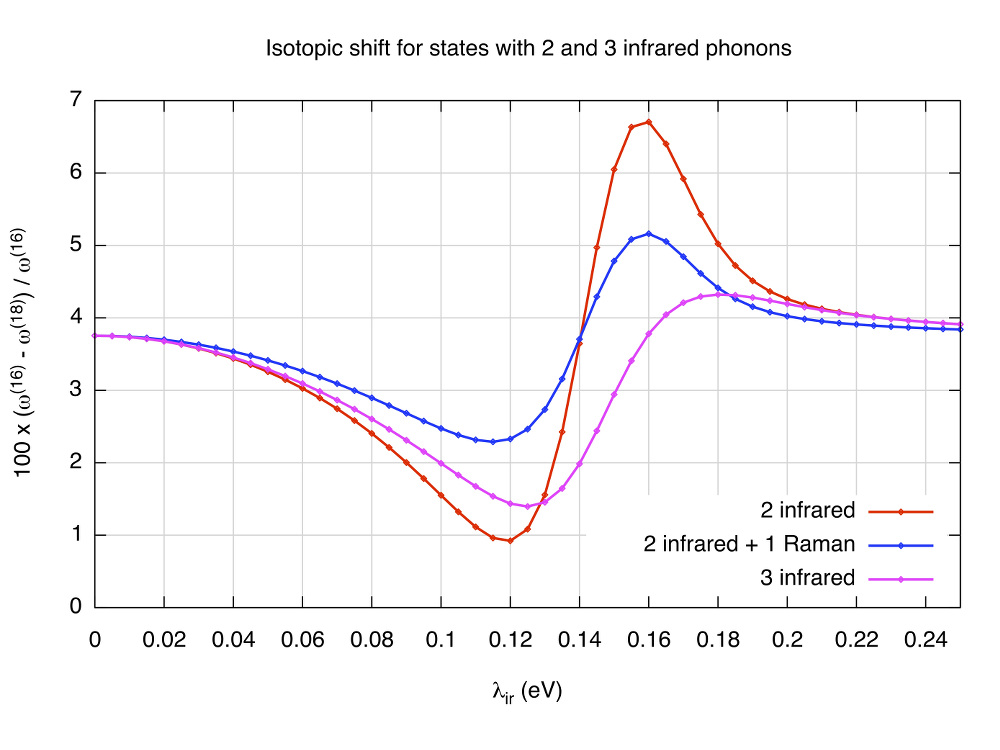
\includegraphics[width=0.8\textwidth]{images/isot-2_3ir.jpg}
  \caption{Isotopic shifts}
  \label{fig:isot-2_3ir}
\end{figure}
